\chapter{Szimulációs eredmények}

Az elkészült szimuláció működésének ellenőrzésére a legegyszerűbb módszer, az általa szolgáltatott eredmények vizsgálata. Helyes működés esetén az így kapott eredmények használhatóak továbbá az ismétlő protokoll pontosabb bemutatására is. Mivel egy általánosított modellt szimulálok,a tesztesetéknél a program felé elvárás az adott esethez várt általános jelleg produkálása. Ennek előzetes meghatározásához használhatjuk az elméleti bevezetőben már megismerteket, valamint  a szakirodalomban megtalálható egyéb szimulációkat, tanulmányokat \cite{briegel1998quantum}\cite{van2009system}\cite{bernardes2011rate}. A vizsgált esetekben, amennyiben nincsen másképp említve, a következő adatokat tekintettem alapértelmezésnek. 
Az összefonódott párok előállításáért felelős állomások 10$\mu s$-ként egyszerre 5 darab 0.7-es tisztaságú párt állítínak elő. Az egyes csatornákra jellemző ``csillapítás hossz'' 20km. A méréseket végző csomópontok mindkét beérkező csatorna felé 20 memória egységgel (összesen 40) rendelkeznek, valamint az egyes mérések előtt 0.98-as előírt tisztaságig tisztíttatják a párokat. Az alapértelmezetten használt tisztító protokoll egy a bevezetőben már ismertetetthez hasonló \cite{deutsch1996quantum} néhány későbbiekben javasolt változtatással \cite{briegel1998quantum}. Ennek lépései a programban teljes egészében, közelítések nélkül vannak szimulálva. Az egyes tisztítások sorrendjének meghatározásához használt alapértelmezett stratégia az ún. ``greedy bottom up '', aminek pontos leírásával majd a későbbiekben foglalkozom. Az egyes mérések elvégzése egy a későbbiekben tárgyalt faszerű struktúra szerint történik. A vizsgált esetek teljesítményét az egységnyi idő alatt sikeresen megosztott párok számával mérjük.

\section{Ismétlő protokoll és az egyszerű csatorna}

Első tesztesetnek azt vizsgáltam milyen távolság fölött kezd egyáltalán előnyt nyújtani a protokoll az ismétlő nélküli csatornával szemben. Tudván, hogy a csatorna átvitele a távolsággal exponenciálisan csökken, míg az ismétlőé csak polinomiálisan \cite{briegel1998quantum} azt várom, hogy kis távolságoknál egyszerűsége miatt a csatorna mutat jobb teljesítmény, míg egy bizonyos távolság felett az ismétlő. Szimulációval 5-500km-es távolságig vizsgáltam az egyes esetek teljesítményét. Először azt az idealizált esetet tekintve, ahol csak a párok elvesztésével kell számolni, a tisztaságukkal nem(szétosztott párok tisztasága = 1), később a csatorna esetén a végpontokban, az ismétlőknél pedig a köztes állomásokon elvégzendő tisztítás hatását is figyelembe véve.
\begin{figure}[H]
\centering
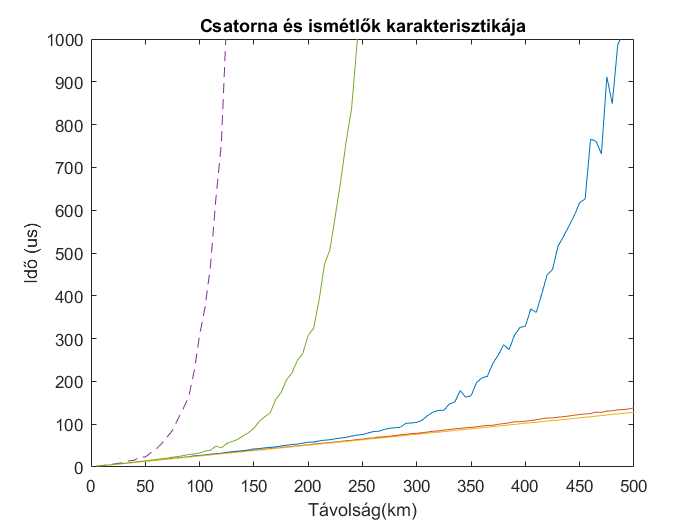
\includegraphics[width=120mm,keepaspectratio]{repvschf1}
\caption[Csatorna és ismétlők karakterisztikája 1]
{Csatorna és különböző ismétlők átvitele a távolság függvényében:\\
Az y tengelyen az egy pár megosztásához szükséges átlagos időt mérjük.\\
Lila szaggatott vonal:egyszerű csatorna.\\
zöld, kék, piros, narancs vonalak: 2, 4, 8 valamint 16, köztes létrehozó állomásból álló ismétlő rendszerek.\\
A szimuláció során kizárólag az átvitel során történő pár vesztést vizsgáltam (megosztott párok tisztasága 1-> nem kell tisztítani).\\
A csatorna és a 2 generátoros rendszer esetében a szimulációt idő előtt leállítottam a veszteségek miatt megnövekedett szükséges számítási kapacitás miatt.
}
\end{figure}
\begin{figure}[H]
\centering
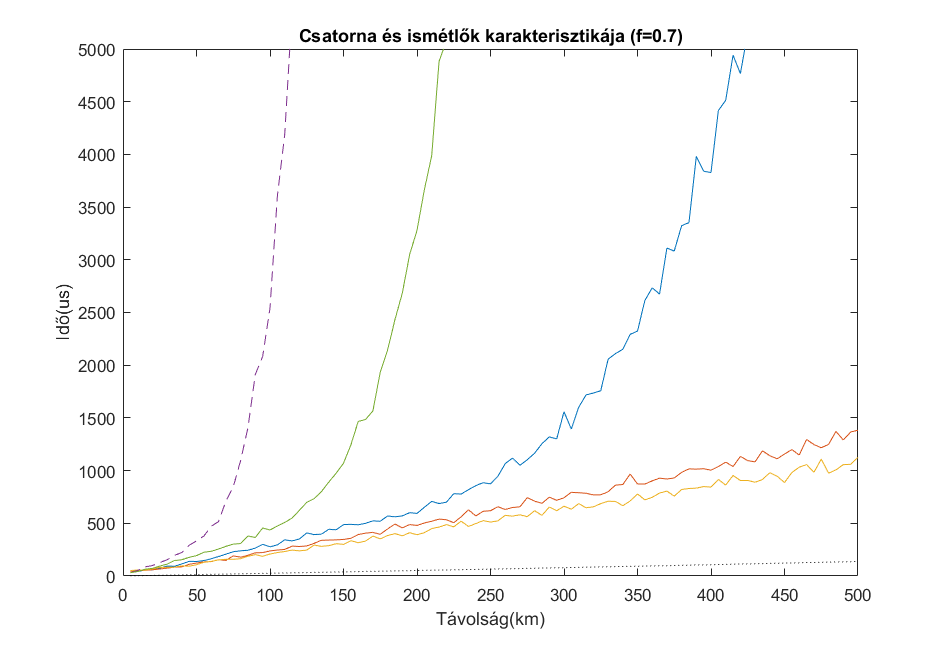
\includegraphics[width=120mm,keepaspectratio]{repvschf07}
\caption[Csatorna és ismétlők karakterisztikája 2]
{Csatorna és különböző ismétlők átvitele a távolság függvényében:\\
Az y tengelyen az egy pár megosztásához szükséges átlagos időt mérjük.\\
Lila szaggatott vonal:egyszerű csatorna.\\
Zöld, kék, piros, narancs vonalak: 2, 4, 8 valamint 16, köztes létrehozó állomásból álló ismétlő rendszerek.\\
Alsó fekete pontozott vonal: 8 köztes állomásból álló rendszer teljes tisztaság esetén.\\
A szétosztott párok ebben az esetben nem ideálisak, a tisztaságuk 0.7-es. Ennek következtében szükség van a tisztító eljárások végrehajtására. (egyszerű csatorna esetében ez a végpontokon történik.)\\
A csatorna és a 2 generátoros rendszer esetében a szimulációt itt is idő előtt leállítottam a veszteségek miatt megnövekedett szükséges számítási kapacitás miatt.
}
\end{figure}
Az egyes esetek teljesítményét az egy pár megosztásához szükséges átlagos idővel mértem (200 megosztott párból számolva).
Látható a csatorna átvitelének exponenciális romlása, valamint nagyobb távolságok esetén az ismétlő elrendezések is ezt a jelleget mutatják. Ennek oka, hogy az egyes állomásokat is exponenciálisan romló csatornák kötik össze. A protokoll fő előnye, hogy egy nagy ilyen szakasz helyett használhatunk több kisebbet. A tisztaság rontásának hatása is megfigyelhető: a teljesen tiszta esethez képest ilyenkor a tisztítás miatt több párt kell felhasználni egy tiszta pár létrehozásához a végpontok között. A görbék jellege nem változott viszont az átlagos idő nőtt.\\
Az ismétlő protokollok természetesen több erőforrást használ mint csupán egy csatorna, viszont ezzel az előzőekben nem foglalkoztam. Ennek figyelembevételre tekintettem a következő eseteket: Álljon rendelkezésre egy 8 generátoros, állomásonként 8x5 memóriaegységgel rendelkező rendszer megvalósításához szükséges erőforráshalmaz. Ebből készíthető egy generátoros esetben egy 8-szor gyorsabb párgenerátor, valamint egyenként 8x5 pár kezelésére alkalmas végpont. Ezen logika mentén elkészíthető még 2 generátoros rendszer, 4-szer gyorsabb generátorokkal és 4x5 memóriával rendelkező állomásokkal, valamint hasonló logika alapján egy 4 generátoros rendszer is. Ezek egymáshoz képesti teljesítménye:
\begin{figure}[H]
\centering
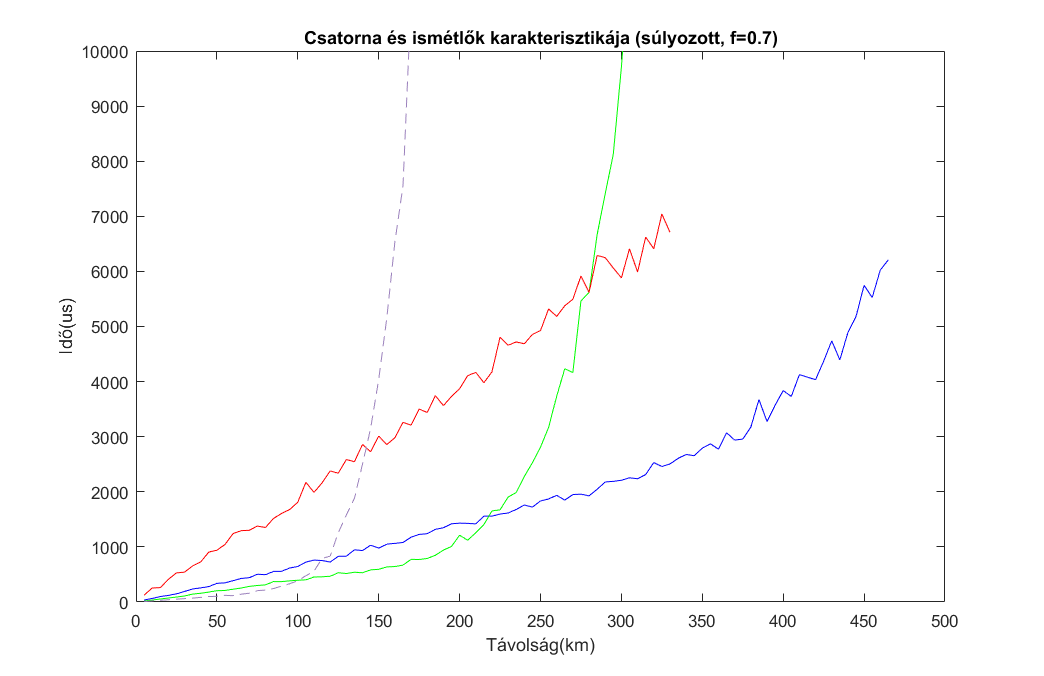
\includegraphics[width=120mm,keepaspectratio]{repvschhandicapped}
\caption[Csatorna és ismétlők karakterisztikája 2]
{Csatorna és különböző ismétlők átvitele a távolság függvényében:\\
Az y tengelyen az egy pár megosztásához szükséges átlagos időt mérjük.\\
Lila szaggatott vonal:egyszerű csatorna.\\
Zöld, kék, piros, vonalak: 2, 4, 8 köztes létrehozó állomásból álló ismétlő rendszerek.\\
A szimulációhoz szükséges idő növekedése miatt, egyes szimulációkat a páronkénti 5000 $\mu s$-os határ elérésénél leállítottam.\\
Az eredményekből látszik, hogy adott erőforrásmennyiség esetén távolságtól függően változik a leggazdaságosabb elrendezés.
}
\end{figure}
Előzetes várakozásoknak megfelelően kis távolságoknál egyszerűsége miatt a csatorna teljesít jobban egészen addig amíg az exponenciális jellegéből származó  veszteségek egy kritikus meg nem haladnak.innentől kezdve először a 2 majd 4 szegmenses ismétlő bizonyul jobbnak. A 8 szegmenses rendszerről a korábbi eredmények jellegének ismeretében feltételezhető, hogy 500-600 km-es távolság esetén már a legjobb alternatívát nyújtja, mivel 500km-hez közelítve a 4 szegmenses elrendezés is exponenciálisan kezd romlani, viszont ezek az értékek már nem tartoznak bele a szimulált tartományba. Ettől eltekintve is látszik a protokoll előnye nagyobb távolságok esetén.

\section{Mérési sorrend}

A protokoll működése során fontos szerepe van az egyes mérések elvégzési sorrendjének is. A következőkben két különböző stratégiát vizsgálok. Az egyik stratégia a többi vizsgálatnál általam alapértelmezettnek használt, ahol a mérések sorrendjét egy faszerű struktúra határozza meg. Itt a hálózat tipikusan $2^n+1$ elemből áll (bár a végpontoknak csak az egyik felét használjuk). Két azonos szinten lévő csomópont között a kapcsolatot mindig a közöttük félúton lévő állomáson elvégzett mérés hozza létre. Ennek megfelelően egy egyszerű hálózatra ez a következőt jelenti:
\begin{figure}[H]
\centering
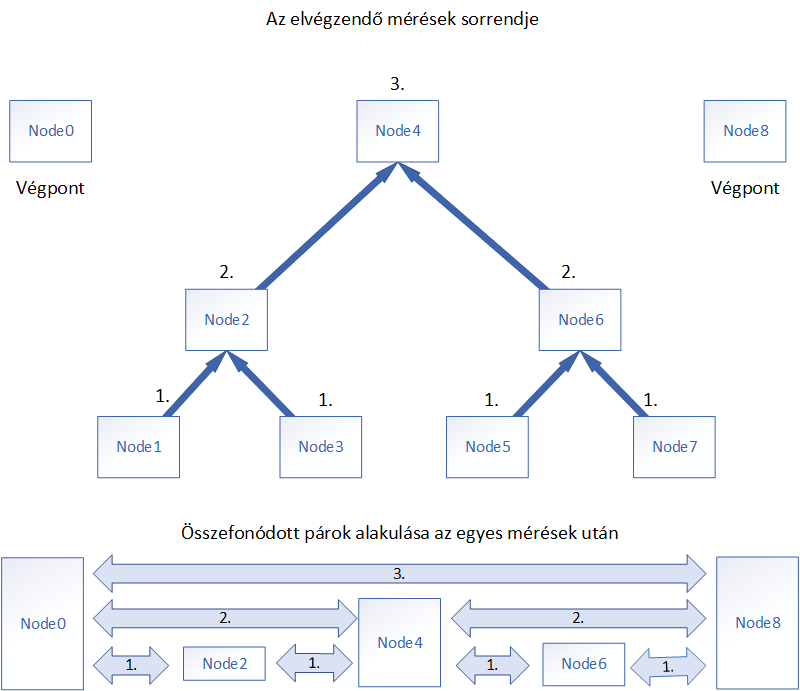
\includegraphics[width=\textwidth,keepaspectratio]{pow2tree}
\caption[Fa alapján történő mérési stratégia]{Az egyes számok a mérések elvégzési sorrendjét jelölik (feltételezzük, hogy minden állomáson rendelkezésre állnak az ehhez szükséges generátorok által küldött párok). A nyilak a sorban következő elvégzendő mérést jelölik, valamint az alsó ábrán az állomások közötti összefonódásokat.}
\end{figure}
Az elrendezésből látszik, hogy ez a stratégia akkor a leghatékonyabb, ha $2^n-1$ közbenső állomás van (+2 végponttal lesz így $2^n+1$ állomás összesen).\\
A másik vizsgált stratégiánál egyszerűen sorban végezzük el a méréseket. Ez a következőképp néz ki:
\begin{figure}[H]
\centering
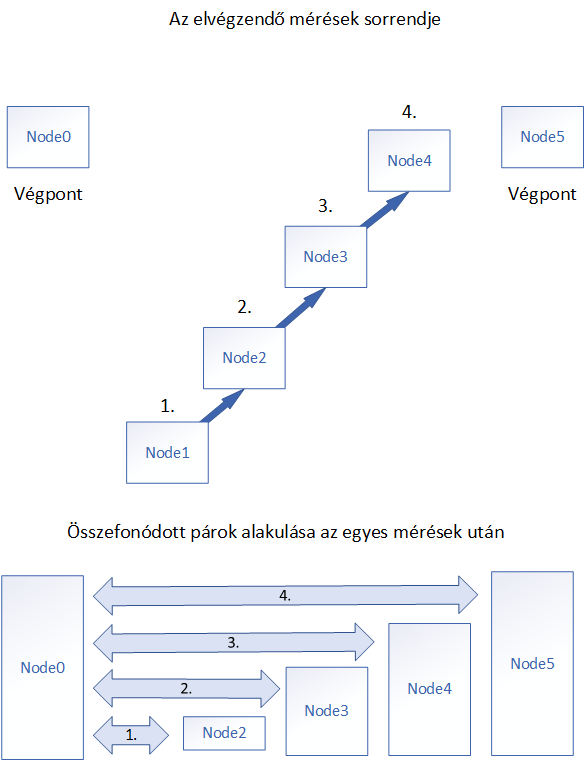
\includegraphics[width=120mm,keepaspectratio]{lintree}
\caption[Egyszerű mérési stratégia]{Az egyes számok itt is a mérések elvégzési sorrendjét jelölik (feltételezzük, hogy minden állomáson rendelkezésre állnak az ehhez szükséges generátorok által küldött párok). A nyilak a sorban következő elvégzendő mérést jelölik, valamint az alsó ábrán az állomások közötti összefonódásokat.}
\end{figure}
\section{Összefonódott pár létrehozási sebesség hatása}

\section{A fogadott párok tisztasága}

\section{Tisztító stratégiák}

\section{Erőforrások elosztása}

\section{Egyéb megfontolandó paraméterek}
\subsection{Protokoll indulása}
Az előzőekben kizárólag a hosszabb működés alatti átlagteljesítményt vizsgáltam, azonban meg kell említeni, hogy a rendszerek rendelkeznek egy úgymond telítődési idővel is ami indulásnál az egyes állomások kezdetben üres memóriáinak megfelelő állapotú párokkal való feltöltődésének ideje. Ennek szemléltetésére vizsgáltam a következőkben az indulástól számított első néhány sikeres megosztásig eltelt időt....

\subsection{Kvantumos memóriák}
Az előzőekben az egyes állomásokon a biteket tároló memóriákat ideálisnak tekintettük, azonban a való életben ezek korántsem azok. Határaik és tökéletlenségeik komoly limitáló tényezőt jelenthetnek. A legjobb tárolási minőségre, valamint a legnagyobb tárolási időre, a végpontokban van szükség, mivel az itt tárolt bitek állapotának fent kell maradni mialatt az összes hozzájuk tartozó mérést elvégezzük. Ennek az időnek az alakulását vizsgálom az alábbi szimulációkban.

